\chapter{Indledning}

Dette 3. semestersprojekt går ud på at udvikle en rugesmaskine.

%Rugesmaskinen skal indeholde en grafisk brugergrænseflade, hvorpå en bruger har mulighed for at betjene systemet. Til denne brugergrænseflade bruges DevKit8000.
%Samtidig skal der benyttes sensorer, som faget I3GFV har givet kendskab til.\newline
%Som bindeled imellem DevKit8000 og de enkelte dele af rugesmaskinen bruges en PSoC 3. Denne PSoC står for at styre selve udrugningssekvensen.

Projektet er underlagt nogle krav, specificeret i det udleverede projektoplæg:

\begin{itemize}
\item Systemet skal via sensorer/aktuatorer interagere med omverdenen
\item Systemet skal have brugerinteraktion
\item Systemet skal indeholde faglige elementer fra semesterets andre fag.
\item Systemet skal anvende DevKit8000 og PSoC3 teknologi.
\end{itemize}

Ydermere er der følgende fokuspunkter:
\begin{itemize}
\item Udarbejdelse af et abstract rettet mod eksterne folk om projektet.
\item Implementering og test af et udviklingsprojekt med både HW og SW, der integrerer semesterets
kurser.
\item Definition af en kravspecifikation for projektet.
\item Samarbejde i grupper med både HW og SW udviklerroller
\item Arbejdsmetode orienteret mod at udvikle nye produkter baseret på HW og SW.
\end{itemize}


%\section{Rapportopbygning}
%Rapporten er bygget op således at de første afsnit giver et overordnet indblik i projektets formål og afgrænsninger. 
%Derefter bliver der sat fokus på kravene for projektet og design overvejelserne.
%I konklusionen på rapporten vil der være en fælles konklusion på projektet. Derudover vil hvert enkelt gruppemedelem komme med hans/hendes personlige konklusion. 
%I starten af rapporten er der inkluderet en ordliste. Denne ordliste er med for at give forståelse for nogen af de begreber der bliver brugt igennem rapporten. 



% \chapter{Tidsplan}

% \begin{figure}[h]
% \centering
% 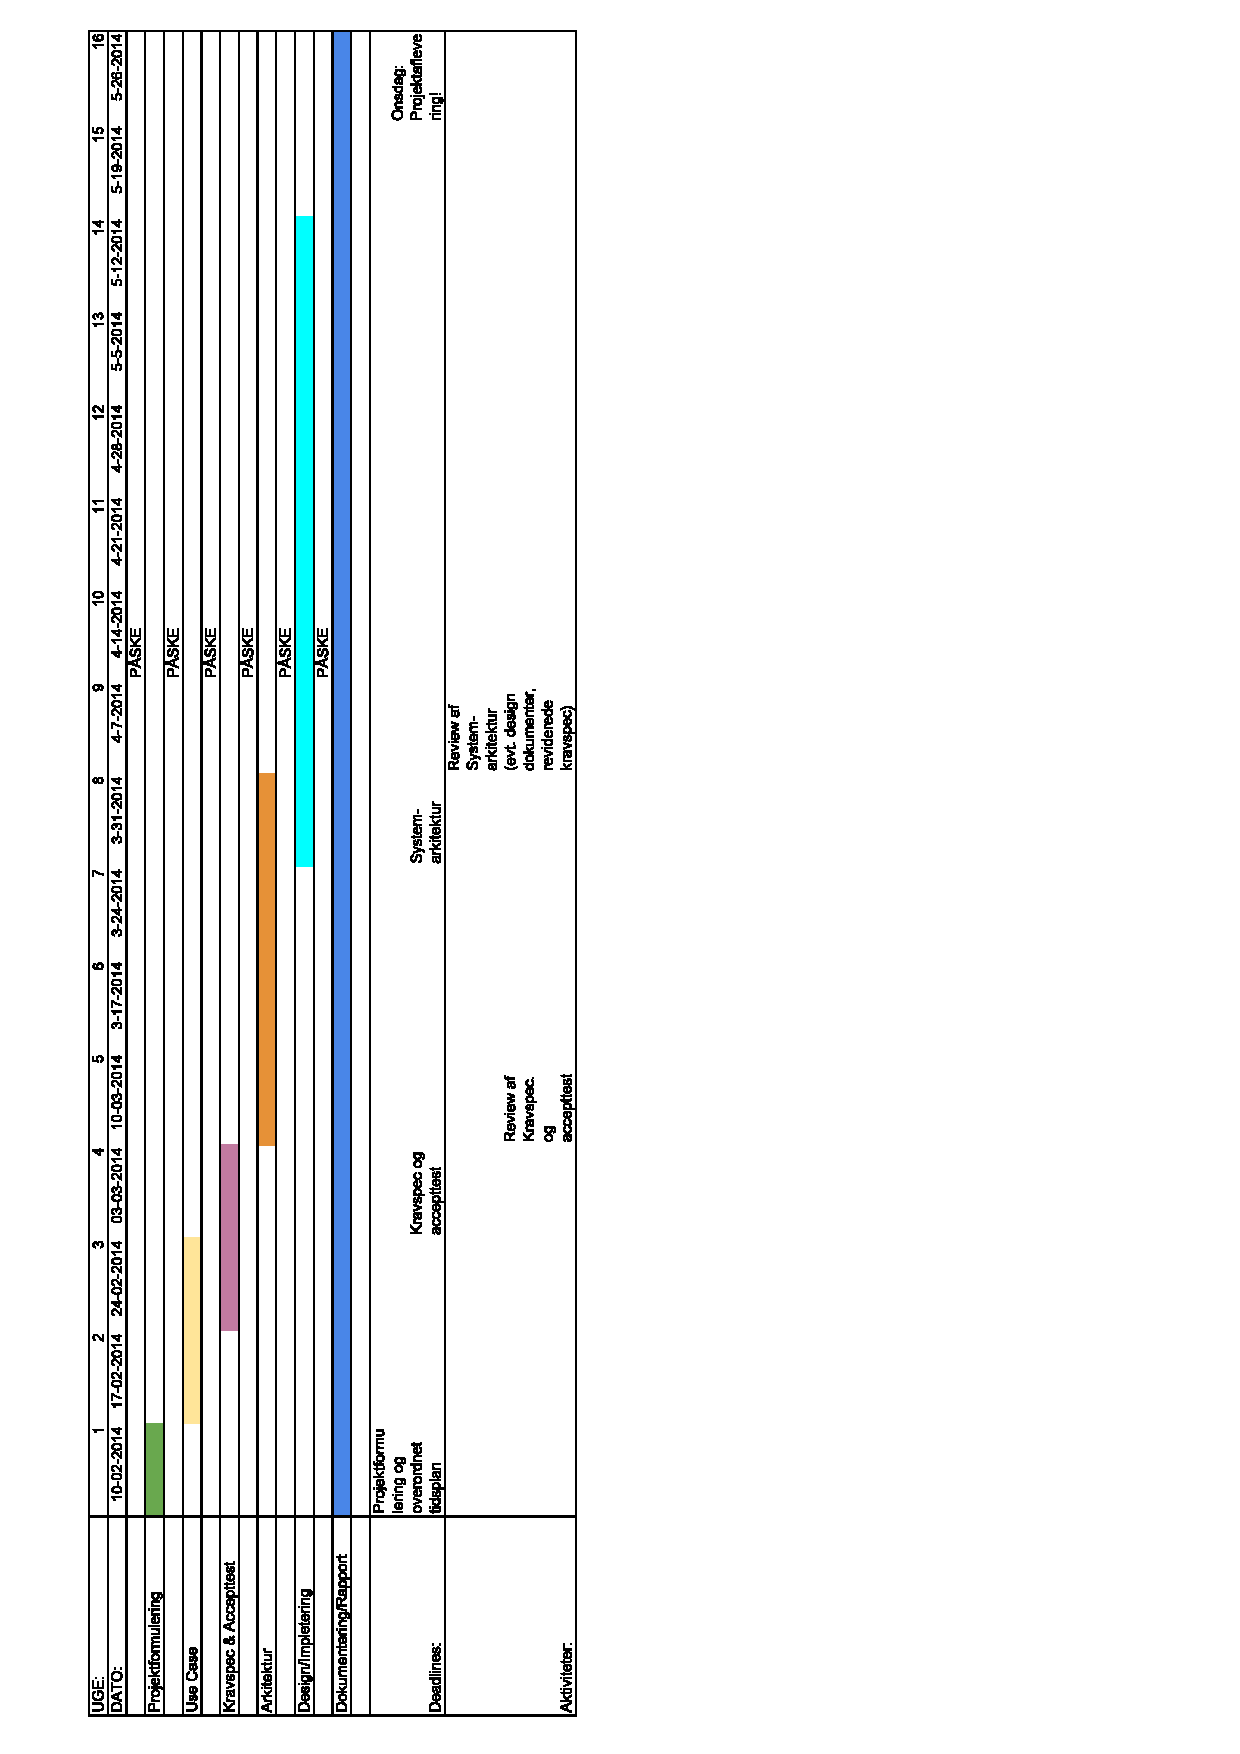
\includegraphics[scale=0.6]{2_indledning/PDFC-.pdf}
% \caption{Skitse af projekt oversigt}
% \label{fig:projektoversigt}
% \end{figure}
% \clearpage

\section{Ordliste}
%\center %affects the entire document???

Denne ordliste er med for at give forståelse for nogen af de begreber der bliver brugt igennem rapporten. 

\begin{tabular}{|l|l|}
\hline  \textbf{Ord} & \textbf{Betydning}  \\ 
\hline SysML & System Modeling Language. \\
\hline Emner & Kyllinger og æg. \\ 
\hline Maskine & Betegner de fysiske rammer. \\
\hline System & Betegner de funktionelle rammer.  \\ 
\hline Ægtype & Typen af æg, der skal udruges. \\
\hline 
\end{tabular} 

\clearpage